\documentclass[•]{article}
\usepackage{amsmath}
\usepackage{graphicx}
\begin{document}
\title{MATLAB Queuing Library}
\author{Juan Felipe Imbett Jim\'enez}
\maketitle
\section{Installation}
The installation of the library is quite easy. Download the .zip file and locate it in the MATLAB root directory. Each .m file must be in your workspace, otherwise MATLAB wont understand the callback. 
\section{Getting started}
The MATLAB Queuing Library consists of the following .m files
\begin{itemize}
\item jacksonNetwork.m Jackson's networks modelling. 
\item mmqueue.m Single queue modelling, with Poisson arrivals and Exponential service times. 
\item pjs.m Subroutine that calculates $P(j \geq s)$ for $M/M/s/GD/\infty / \infty$
\end{itemize}
\section{mmqueue.m}
This file calculates the values of $L,L_q,L_s,W,W_q,W_s$ for a queue with exponentially distributed inter arrival times and service times. The command is the following: \bigskip
\begin{equation}
[L,L_q,L_s,W,W_q,W_s]=mmqueue(s, \lambda, \mu, c)
\end{equation}
Where $s$ is the number of servers, $\lambda$ is the arrival rate, $\mu$ is the service rate and $c$ is the capacity. If the system has an infinite capacity $c=-1$. The following example shows the routine:
\begin{itemize}
\item System: $M/M/1/GD/5 / \infty$
\item $\lambda=5$
\item $\mu=4$ 
\end{itemize}
\bigskip
 The code in MATLAB is the following:

 \begin{center}
 \begin{figure}
 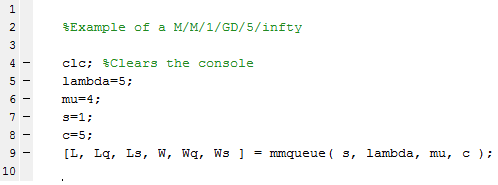
\includegraphics[scale=0.8]{Example1.png}
 \end{figure}
 \end{center}
  
  \begin{center}
 \begin{figure}
 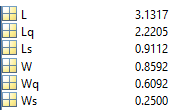
\includegraphics[scale=1]{ResultsExample1.png}
 \end{figure}
 \end{center}
 
 \section{jacksonNetwork.m}
 This file calculates $L,L_q,L_s,W,W_q,W_s$ for a Jackson's Network. If any assumption is violated the routine handles an error. The command is the following:
 \begin{equation}
 [L,L_q,L_s,W,W_q,W_s]=jacksonNetwork( \gamma, P , s, \mu)
 \end{equation}
 Where $\gamma$ is a row vector with the external arrival rates, $P$ is the transition probability between stations, $s$ is a row vector with the number of servers in each station, if the number of servers is infinite then $s=-1$, and $\mu$ is a row vector with service rates in each station. Consider the following example of a Jackson's network:
 \begin{itemize}
 \item 3 stations
 \item $\gamma = [2,3,0]$
 \item $P_{1,3}=1,  P_{2,1}=\frac{1}{2},P_{2,3}=\frac{1}{2} , P_{3,2} = \frac{1}{2}$
 \item $s=[1,2,\infty]$
 \item $\mu=[10,15,2]$
\end{itemize}
The code in MATLAB is the following:

 \begin{figure}
 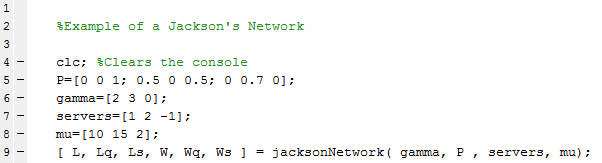
\includegraphics[scale=0.8]{Example2.png}
 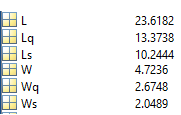
\includegraphics[scale=1]{ResultsExample2.png}
 \end{figure}
 


\end{document}